%%% Local Variables:
%%% mode: latex
%%% TeX-master: t
%%% End:

\section{Metamask, The Wallet Auth}

To transact on Ethereum, you need an account. There is no MySQL ``users'' table. There is no email/password login. \\[-8pt]

To create an Ethereum account, you need to set up a crypto wallet like Metamask. The wallet will be responsible for generating and securing your crypto keys for signing transactions. \\[-8pt]

Metamask generates your Private Key. You derive the Public Key from the Private Key. Your account's address is the last 20 bytes of a hashed Public Key. \\[-8pt]

\namedfigure
{!hbtp}
{img:scdsaGenKey}
{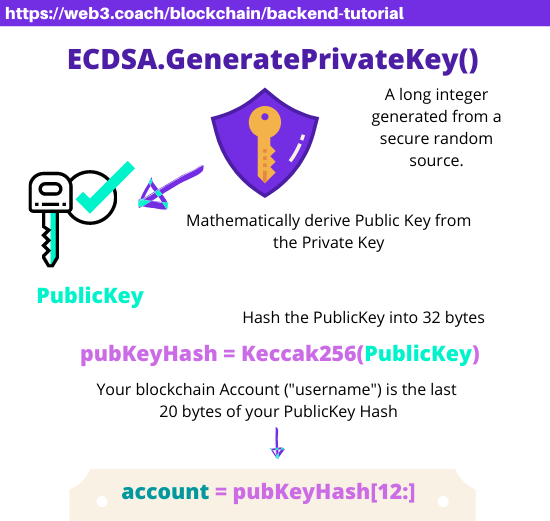
\includegraphics[width=\textwidth]{ecdsa_generate_key.png}}
{Generating keys and addresses.}


The JS libraries will then connect to your Metamask wallet (if you permit them to do so), and they will ask you to sign Ethereum transactions. A decentralized application can't do anything without your signature.

Figure \ref{img:transactionFlowDig} show the transaction flow diagram.

\namedfigure
{!hbtp}
{img:transactionFlowDig}
{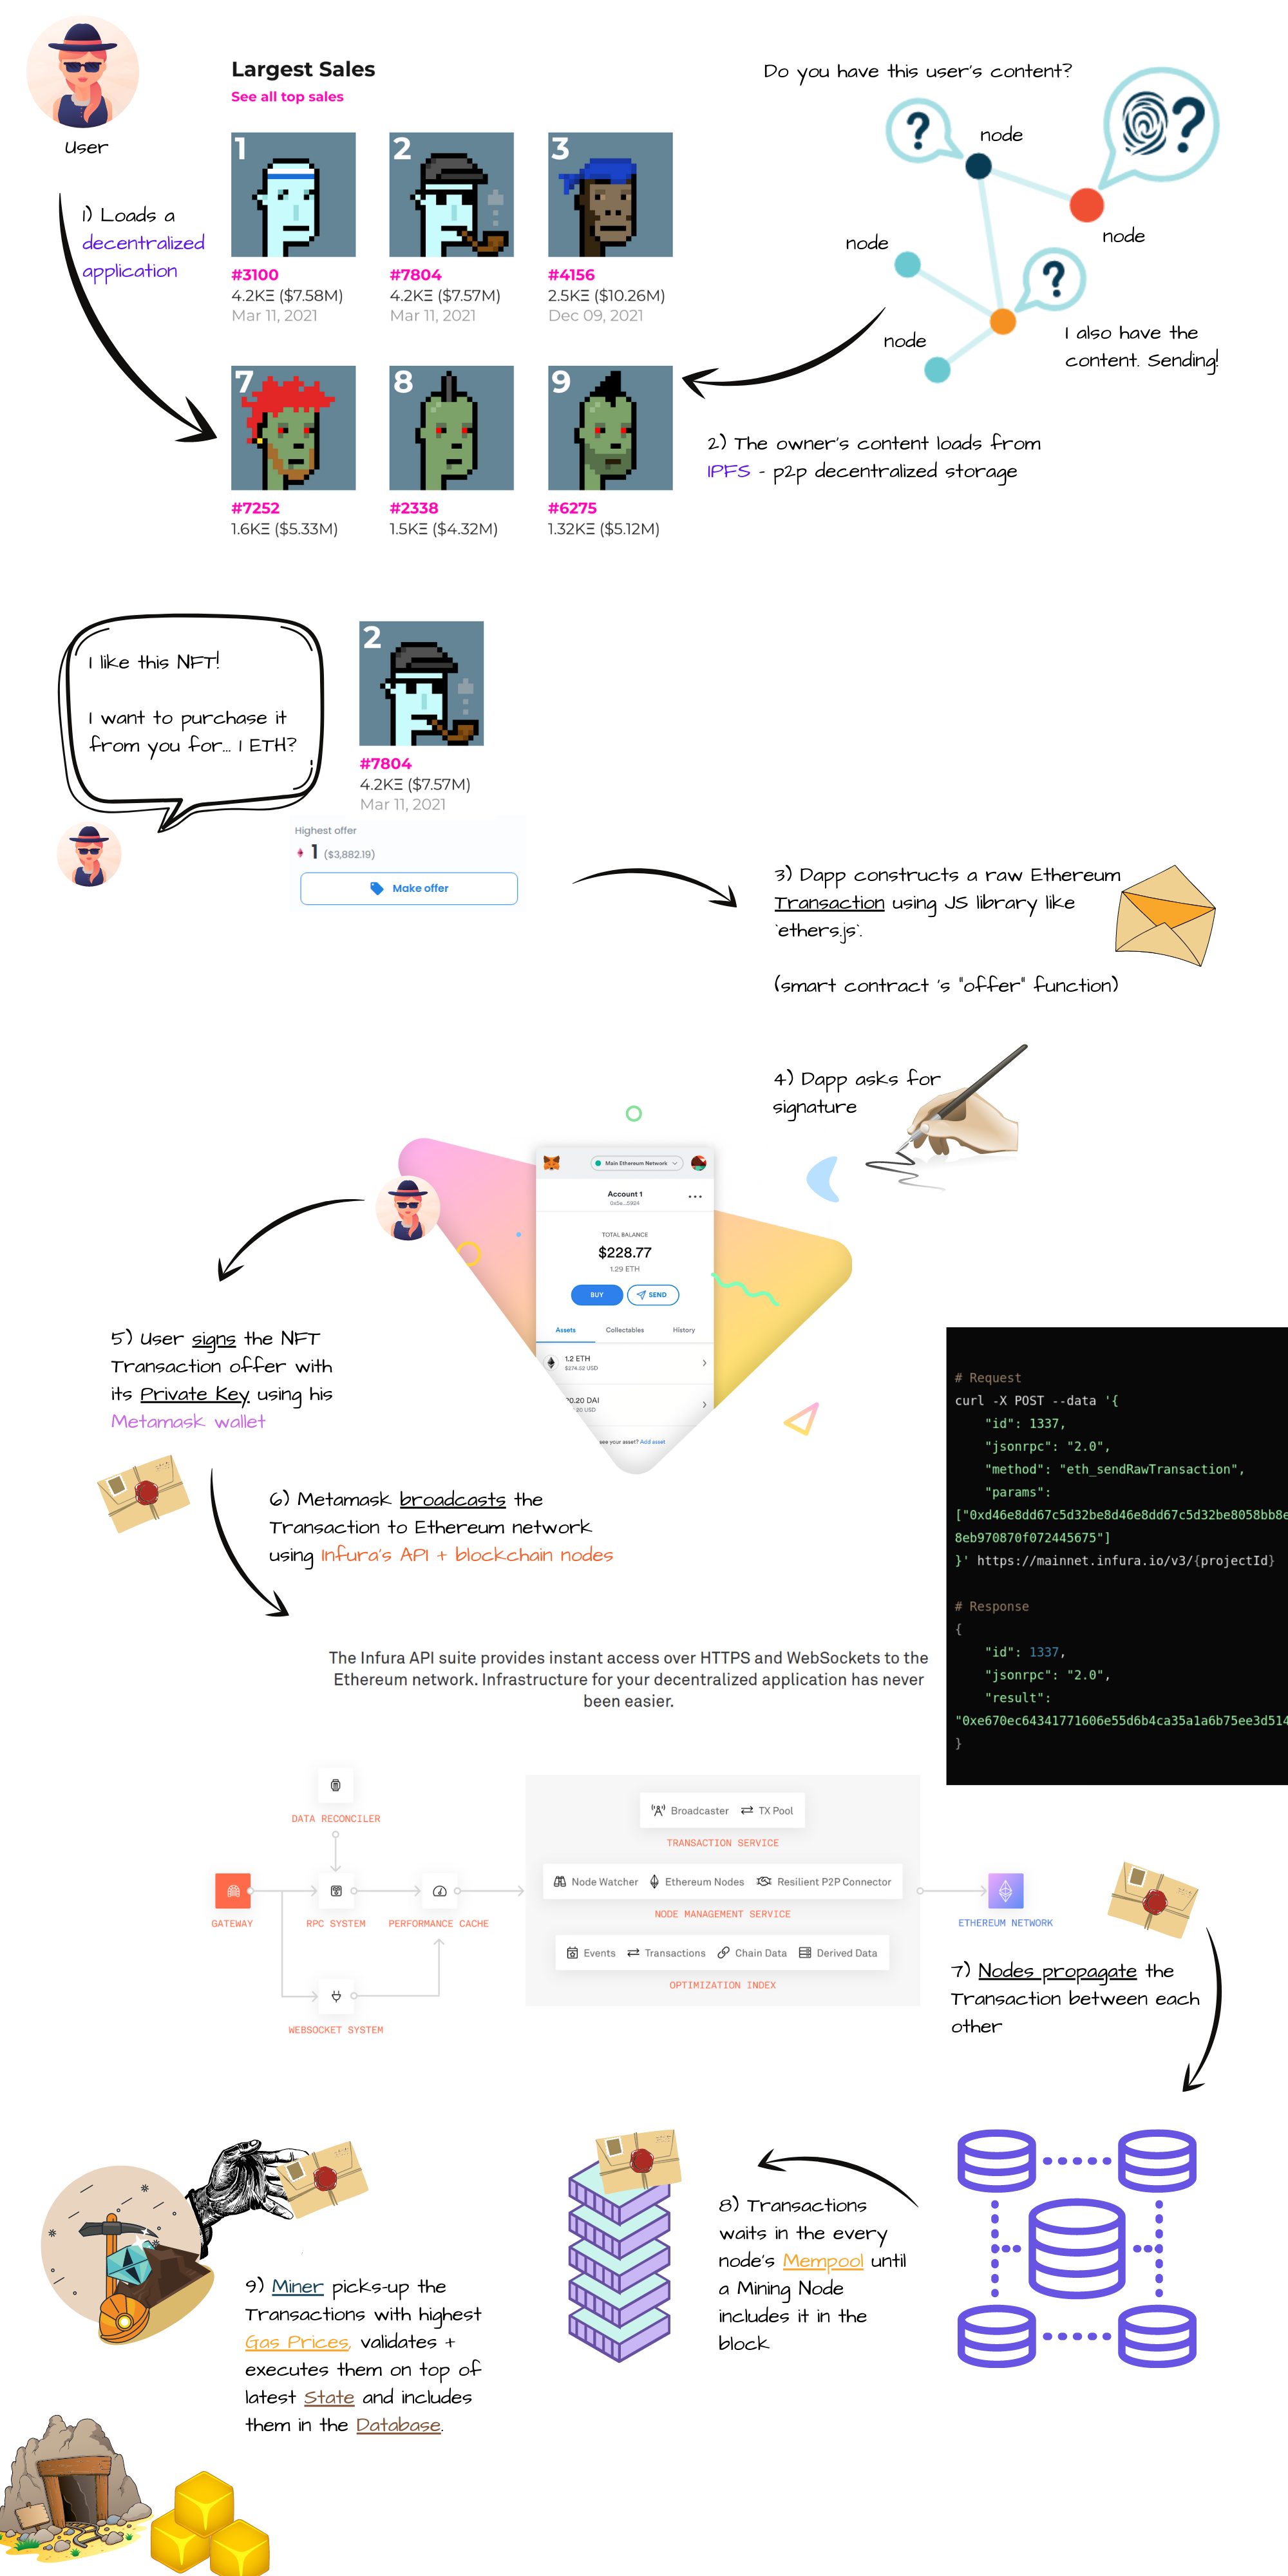
\includegraphics[width=0.7\textwidth]{transaction_flow_dig.png}}
{Transaction flow diagram.}
